\documentclass[25pt, a0paper, landscape, blockverticalspace=12mm, colspace=12mm]{tikzposter}
\usepackage{polyglossia} %% загружает пакет многоязыковой вёрстки
\setdefaultlanguage{russian}
\setotherlanguage{english} 
\defaultfontfeatures{Ligatures={TeX},Renderer=Basic}
\usepackage{libertine}
\usepackage[scaled=0.92]{inconsolata}
\usepackage[libertine]{newtxmath}
\usepackage{wrapfig}
\usepackage{array,graphicx,caption}
\usepackage{lipsum}
\usepackage[]{color}
\newfontfamily{\cyrillicfonttt}{Courier New}




\title{Алгоритмы кластеризации}
\author{Корышева Юлия; Переверзев Виктор; Ляшев Глеб}
\date{\today}
\institute{Факультет экономических наук НИУ ВШЭ}
 
\usetheme{Autumn}
\definecolor{myOrange}{rgb}{0.97, 0.91, 0.81}
\colorlet{backgroundcolor}{myOrange} 
\begin{document}
 
\maketitle  
 
\begin{columns}

\column{0.23}
    \block{\textcolor{black}{k-means}}{

Алгоритм разбивает объекты на заранее известное число кластеров, при условии минимизации среднего расстояния между каждым объектом кластера и его центроидом. 

\begin{enumerate}
\item На первом шаге фиксируются стартовые центроиды.   


\[
\begin{tikzpicture}
    \begin{scope}[yshift=-7.5cm, xshift=7.5cm]
        \draw (-3.5, 3.5 ) -- (3.5, 3.5);
        \draw (-3.5, -3.5) -- (3.5, -3.5);
        \draw (-3.5, -3.5) -- (-3.5, 3.5);
        \draw (3.5, 3.5) -- (3.5, -3.5);

        \draw[blue, fill=blue] (-1.5, -2.5) circle (0.2);
        \draw[blue, fill=blue] (-1.75, -0.5) circle (0.2);
        \draw[blue, fill=blue] (-1.5, 1.4) circle (0.2);
        \draw[blue, fill=blue] (-2, 0.75) circle (0.2);
        \draw[blue, fill=blue] (-2.625, 1.8) circle (0.2);
        \draw[blue, fill=blue] (1.75, -3.2) circle (0.2);
        \draw[blue, fill=blue] (3, -2.8) circle (0.2);
        \draw[blue, fill=blue] (3, -0.5) circle (0.2);
        \draw[blue, fill=blue] (1.75, -0.5) circle (0.2);
        \draw[blue, fill=blue] (2.7, 1.2) circle (0.2);
        \draw[blue, fill=blue] (2.5, 1.8) circle (0.2);
        \draw[blue, fill=blue] (0.5, 1) circle (0.2);
        \draw[blue, fill=blue] (-0.4, 2.3) circle (0.2);
        \draw[blue, fill=blue] (-0.9, 2.9) circle (0.2); 
        \draw[black] (-3, 1.5) -- (-2.5, 1);
        \draw[black] (-3, 1) -- (-2.5, 1.5);
        \draw[black] (0.25, 3) -- (0.75, 3.5);
        \draw[black] (0.25, 3.5) -- (0.75, 3);
        \filldraw[black](0.5, 3.25) circle (2pt);
        \filldraw[black] (-2.75 , 1.25) circle (2pt);
    \end{scope}
\end{tikzpicture}
\]
 
\item На втором шаге объекты разбиваются на кластеры, при условии минимизации расстояния от объектов до центроида. 

\[
\begin{tikzpicture}
    \begin{scope}[xshift=7.5cm, yshift=7.5cm]
        \draw (-3.5, 3.5 ) -- (3.5, 3.5);
        \draw (-3.5, -3.5) -- (3.5, -3.5);
        \draw (-3.5, -3.5) -- (-3.5, 3.5);
        \draw (3.5, 3.5) -- (3.5, -3.5);

        \draw[red, fill=red] (-1.5, -2.5) circle (0.2);
        \draw[red, fill=red] (-1.75, -0.5) circle (0.2);
        \draw[red, fill=red] (-1.5, 1.4) circle (0.2);
        \draw[red, fill=red] (-2, 0.75) circle (0.2);
        \draw[red, fill=red] (-2.625, 1.8) circle (0.2);
        \draw[yellow, fill=yellow] (1.75, -3.2) circle (0.2);
        \draw[yellow, fill=yellow] (3, -2.8) circle (0.2);
        \draw[yellow, fill=yellow] (3, -0.5) circle (0.2);
        \draw[yellow, fill=yellow] (1.75, -0.5) circle (0.2);
        \draw[yellow, fill=yellow] (2.7, 1.2) circle (0.2);
        \draw[yellow, fill=yellow] (2.5, 1.8) circle (0.2);
        \draw[yellow, fill=yellow] (0.5, 1) circle (0.2);
        \draw[yellow, fill=yellow] (-0.4, 2.3) circle (0.2);
        \draw[yellow, fill=yellow] (-0.9, 2.9) circle (0.2); 
        \draw[black] (-3, 1.5) -- (-2.5, 1);
        \draw[black] (-3, 1) -- (-2.5, 1.5);
        \draw[black] (0.25, 3) -- (0.75, 3.5);
        \draw[black] (0.25, 3.5) -- (0.75, 3);
        \draw[black] (1.5, -3.4) -- (-1.5, 3.4);
        \filldraw[black](0.5, 3.25) circle (2pt);
        \filldraw[black] (-2.75 , 1.25) circle (2pt);

        
    \end{scope}
\end{tikzpicture}
\]

\item Алгоритм пересчитывает значения центроидов.

\[
\begin{tikzpicture}
    \begin{scope}[xshift=7.5cm, yshift=7.5cm]
        \draw (-3.5, 3.5 ) -- (3.5, 3.5);
        \draw (-3.5, -3.5) -- (3.5, -3.5);
        \draw (-3.5, -3.5) -- (-3.5, 3.5);
        \draw (3.5, 3.5) -- (3.5, -3.5);

        \draw[red, fill=red] (-1.5, -2.5) circle (0.2);
        \draw[red, fill=red] (-1.75, -0.5) circle (0.2);
        \draw[red, fill=red] (-1.5, 1.4) circle (0.2);
        \draw[red, fill=red] (-2, 0.75) circle (0.2);
        \draw[red, fill=red] (-2.625, 1.8) circle (0.2);
        \draw[yellow, fill=yellow] (1.75, -3.2) circle (0.2);
        \draw[yellow, fill=yellow] (3, -2.8) circle (0.2);
        \draw[yellow, fill=yellow] (3, -0.5) circle (0.2);
        \draw[yellow, fill=yellow] (1.75, -0.5) circle (0.2);
        \draw[yellow, fill=yellow] (2.7, 1.2) circle (0.2);
        \draw[yellow, fill=yellow] (2.5, 1.8) circle (0.2);
        \draw[yellow, fill=yellow] (0.5, 1) circle (0.2);
        \draw[yellow, fill=yellow] (-0.4, 2.3) circle (0.2);
        \draw[yellow, fill=yellow] (-0.9, 2.9) circle (0.2); 
        \draw[black] (1.5, -3.4) -- (-1.5, 3.4);
        \draw[->][black] (-2.75, 0.9) -- (-2.3, 0.1);
        \draw[->][black] (0.5, 2.9) -- (1.2, 0.75);
        \draw[black] (-3, 1.5) -- (-2.5, 1);
        \draw[black] (-3, 1) -- (-2.5, 1.5);
        \draw[black] (0.25, 3) -- (0.75, 3.5);
        \draw[black] (0.25, 3.5) -- (0.75, 3);
        \filldraw[black](0.5, 3.25) circle (2pt);
        \filldraw[black] (-2.75 , 1.25) circle (2pt);
        \draw[black] (-2.5, -0.5) -- (-2, 0);
        \draw[black] (-2, -0.5) -- (-2.5, 0);
        \filldraw[black](-2.25, -0.25) circle (2pt);
        
        \draw[black] (1, 0.2) -- (1.5, 0.7);
        \draw[black] (1.5, 0.2) -- (1, 0.7);
        \filldraw[black](1.25, 0.45) circle (2pt);
        
    \end{scope}
\end{tikzpicture}
\]

\item Алгоритм выполняет шаги 2-3 до тех пор, пока кластеры будут изменяться. 
 

\begin{tikzpicture}
        \begin{scope}
        \draw (-3.5, 3.5 ) -- (3.5, 3.5);
        \draw (-3.5, -3.5) -- (3.5, -3.5);
        \draw (-3.5, -3.5) -- (-3.5, 3.5);
        \draw (3.5, 3.5) -- (3.5, -3.5);
    
        \draw[red, fill=red] (-1.5, -2.5) circle (0.2);
        \draw[red, fill=red] (-1.75, -0.5) circle (0.2);
        \draw[red, fill=red] (-1.5, 1.4) circle (0.2);
        \draw[red, fill=red] (-2, 0.75) circle (0.2);
        \draw[red, fill=red] (-2.625, 1.8) circle (0.2);
        \draw[yellow, fill=yellow] (1.75, -3.2) circle (0.2);
        \draw[yellow, fill=yellow] (3, -2.8) circle (0.2);
        \draw[yellow, fill=yellow] (3, -0.5) circle (0.2);
        \draw[yellow, fill=yellow] (1.75, -0.5) circle (0.2);
        \draw[yellow, fill=yellow] (2.7, 1.2) circle (0.2);
        \draw[yellow, fill=yellow] (2.5, 1.8) circle (0.2);
        \draw[yellow, fill=yellow] (0.5, 1) circle (0.2);
        \draw[red, fill=red] (-0.4, 2.3) circle (0.2);
        \draw[red, fill=red] (-0.9, 2.9) circle (0.2); 
 

        \draw[black] (0.5, 3.4) -- (-1.5, -3.4);
        \draw[->][black] (-2.25, 0) -- (-1.8, 1);
        \draw[->][black] (1.3, 0.1) -- (1.9, -0.4);
        \draw[black] (-2.5, -0.5) -- (-2, 0);
        \draw[black] (-2, -0.5) -- (-2.5, 0);
        \filldraw[black](-2.25, -0.25) circle (2pt);
        \draw[black] (1, 0.2) -- (1.5, 0.7);
        \draw[black] (1.5, 0.2) -- (1, 0.7);
        \filldraw[black](1.25, 0.45) circle (2pt);
        

        \draw[black] (-2, 1) -- (-1.5, 1.5);
        \draw[black] (-1.5, 1) -- (-2, 1.5);
        \filldraw[black](-1.75, 1.25) circle (2pt);
        
        
        \draw[black] (1.75, -1) -- (2.25, -0.5);
        \draw[black] (2.25, -1) -- (1.75, -0.5);
        \filldraw[black](2, -0.75) circle (2pt);
        
        

    \end{scope}

  \begin{scope}[xshift=15cm]
        \draw (-3.5, 3.5 ) -- (3.5, 3.5);
        \draw (-3.5, -3.5) -- (3.5, -3.5);
        \draw (-3.5, -3.5) -- (-3.5, 3.5);
        \draw (3.5, 3.5) -- (3.5, -3.5);
    
        \draw[yellow, fill=yellow] (-1.5, -2.5) circle (0.2);
        \draw[red, fill=red] (-1.75, -0.5) circle (0.2);
        \draw[red, fill=red] (-1.5, 1.4) circle (0.2);
        \draw[red, fill=red] (-2, 0.75) circle (0.2);
        \draw[red, fill=red] (-2.625, 1.8) circle (0.2);
        \draw[yellow, fill=yellow] (1.75, -3.2) circle (0.2);
        \draw[yellow, fill=yellow] (3, -2.8) circle (0.2);
        \draw[yellow, fill=yellow] (3, -0.5) circle (0.2);
        \draw[yellow, fill=yellow] (1.75, -0.5) circle (0.2);
        \draw[yellow, fill=yellow] (2.7, 1.2) circle (0.2);
        \draw[yellow, fill=yellow] (2.5, 1.8) circle (0.2);
        \draw[red, fill=red] (0.5, 1) circle (0.2);
        \draw[red, fill=red] (-0.4, 2.3) circle (0.2);
        \draw[red, fill=red] (-0.9, 2.9) circle (0.2); 

        \draw[blue] (3, 3.4) -- (-2.8, -3.4);

        \draw[black] (-1, 1.5) -- (-0.5, 2);
        \draw[black] (-0.5, 1.5) -- (-1, 2);
        \filldraw[black](-0.75, 1.75) circle (2pt);
        
        
        \draw[black] (1.5, -1.5) -- (2, -1);
        \draw[black] (2, -1.5) -- (1.5, -1);
        \filldraw[black](1.75, -1.25) circle (2pt);

        
        \end{scope}
        
 \begin{scope}[xshift=7.5cm]
        \draw (-3.5, 3.5 ) -- (3.5, 3.5);
        \draw (-3.5, -3.5) -- (3.5, -3.5);
        \draw (-3.5, -3.5) -- (-3.5, 3.5);
        \draw (3.5, 3.5) -- (3.5, -3.5);
    
        \draw[yellow, fill=yellow] (-1.5, -2.5) circle (0.2);
        \draw[red, fill=red] (-1.75, -0.5) circle (0.2);
        \draw[red, fill=red] (-1.5, 1.4) circle (0.2);
        \draw[red, fill=red] (-2, 0.75) circle (0.2);
        \draw[red, fill=red] (-2.625, 1.8) circle (0.2);
        \draw[yellow, fill=yellow] (1.75, -3.2) circle (0.2);
        \draw[yellow, fill=yellow] (3, -2.8) circle (0.2);
        \draw[yellow, fill=yellow] (3, -0.5) circle (0.2);
        \draw[yellow, fill=yellow] (1.75, -0.5) circle (0.2);
        \draw[yellow, fill=yellow] (2.7, 1.2) circle (0.2);
        \draw[yellow, fill=yellow] (2.5, 1.8) circle (0.2);
        \draw[red, fill=red] (0.5, 1) circle (0.2);
        \draw[red, fill=red] (-0.4, 2.3) circle (0.2);
        \draw[red, fill=red] (-0.9, 2.9) circle (0.2); 

        \draw[->][black] (-1.4, 1.2) -- (-0.85, 1.4);
        \draw[->][black] (1.9, -0.95) -- (1.75, -1.1);
        \draw[blue] (3, 3.4) -- (-2.5, -3.4);
                
        \draw[black] (-1, 1.5) -- (-0.5, 2);
        \draw[black] (-0.5, 1.5) -- (-1, 2);
        \filldraw[black](-0.75, 1.75) circle (2pt);
        
        
        \draw[black] (1.5, -1.5) -- (2, -1);
        \draw[black] (2, -1.5) -- (1.5, -1);
        \filldraw[black](1.75, -1.25) circle (2pt);
        
        \draw[black] (-2, 1) -- (-1.5, 1.5);
        \draw[black] (-1.5, 1) -- (-2, 1.5);
        \filldraw[black](-1.75, 1.25) circle (2pt);
        
        
        \draw[black] (1.75, -1) -- (2.25, -0.5);
        \draw[black] (2.25, -1) -- (1.75, -0.5);
        \filldraw[black](2, -0.75) circle (2pt);
    \end{scope}

  
\end{tikzpicture}

\end{enumerate}
}
\block{\textcolor{black}{Начальные центроиды}}{
Выбор начальных центроидов может осуществляться следующим образом:
\begin{itemize}
    \item Случайный выбор k-объектов. 
    \item Выбор первых k-объектов. 
\end{itemize}
}

\column{0.21}
    \block{\textcolor{black}{DBSCAN}}{Суть работы алгоритма заключается в захвате кластеров через соседние точки. При заданном минимальном расстоянии для захвата и минимальном количестве точек для создания кластеров захваченным объектам присваиваются метки кластера или иначе же метки выбросов.
\begin{enumerate}
      \item DBSCAN нашел случайную точку $A$ в пространстве и «заразил» ее. Далее происходит последовательный захват соседей ($B$, $C$, $D$), находящихся друг от друга в пределах требуемого расстояния.  
      
\[
\begin{tikzpicture}
\tikzset{every node}=[font=\small]
    \draw (-3.5, 3.5) -- (3.5, 3.5);
    \draw (-3.5, -3.5) -- (3.5, -3.5);
    \draw (-3.5, -3.5) -- (-3.5, 3.5);
    \draw (3.5, 3.5) -- (3.5, -3.5);
        
    \draw[red, fill=red] (2.5, 2.5) circle (0.12) node[above, color=black]{$A$};
    \draw (1.35, 2.25) circle (0.12) node[above]{$D$};
    \draw (1.6, 1.1) circle (0.12) node[above]{$C$};
    \draw (1.95, 1.9) circle (0.12) node[above]{$B$};
    \draw (-2.4, -1.9) circle (0.12);
    \draw (-1.8, -1.3) circle (0.12);
    \draw (-1.95, 2.11) circle (0.12);
    \draw (2.6, -2.4) circle (0.12);
        
    \draw[->][red] (2.435, 2.435) -- (2.04, 2.01);
    \draw[->][red] (1.88, 1.77) -- (1.64, 1.23);
    \draw[->][red] (1.82, 1.96) -- (1.47, 2.18);
\end{tikzpicture}
\]
    
    \item Когда все цели поражены, на захваченных территориях DBSCAN принимает решение создать тоталитарное государство-кластер. Но и этого ему мало. Следующим что на пути безжалостной машины попался объект $E$.
    
    \[
\begin{tikzpicture}
\tikzset{every node}=[font=\small]
    \draw (-3.5, 3.5) -- (3.5, 3.5);
    \draw (-3.5, -3.5) -- (3.5, -3.5);
    \draw (-3.5, -3.5) -- (-3.5, 3.5);
    \draw (3.5, 3.5) -- (3.5, -3.5);
        
    \draw[red, fill=red] (2.5, 2.5) circle (0.12);
    \draw[red, fill=red] (1.35, 2.25) circle (0.12);
    \draw[red, fill=red] (1.6, 1.1) circle (0.12);
    \draw[red, fill=red] (1.95, 1.9) circle (0.12);
    \draw (-2.4, -1.9) circle (0.12);
    \draw (-1.8, -1.3) circle (0.12);
    \draw[green, fill=green] (-1.95, 2.11) circle (0.12) node[above, color=black]{$E$};
    \draw (2.6, -2.4) circle (0.12);
        
    \draw[<->][red] (2.435, 2.435) -- (2.04, 2.01);
    \draw[<->][red] (1.88, 1.77) -- (1.64, 1.23);
    \draw[<->][red] (1.82, 1.96) -- (1.47, 2.18);
    \draw[<->][red] (1.54, 1.24) -- (1.30, 2.13);
    \draw[<->][red] (1.74, 1.19) -- (2.5, 2.36);
    \draw[<->][red] (1.47, 2.27) -- (2.37, 2.5);
\end{tikzpicture}
\]
    
\item Найдя точку $G$ рядом c соседом $F$, алгоритм захватывает эти два объекта и присваивает им метку кластера. Снова запускается поиск.
    
\[
\begin{tikzpicture}
\tikzset{every node}=[font=\small]
        \draw (-3.5, 3.5) -- (3.5, 3.5);
        \draw (-3.5, -3.5) -- (3.5, -3.5);
        \draw (-3.5, -3.5) -- (-3.5, 3.5);
        \draw (3.5, 3.5) -- (3.5, -3.5);
        
        \draw[red, fill=red] (2.5, 2.5) circle (0.12);
        \draw[red, fill=red] (1.35, 2.25) circle (0.12);
        \draw[red, fill=red] (1.6, 1.1) circle (0.12);
        \draw[red, fill=red] (1.95, 1.9) circle (0.12);
        \draw (-2.4, -1.9) circle (0.12) node[above, color=black]{$G$};
        \draw[blue, fill=blue] (-1.8, -1.3) circle (0.12) node[above, color=black]{$F$};
        \draw[green, fill=green] (-1.95, 2.11) circle (0.12);
        \draw (2.6, -2.4) circle (0.12);
        
        \draw[->][red] (2.435, 2.435) -- (2.04, 2.01);
        \draw[->][red] (1.88, 1.77) -- (1.64, 1.23);
        \draw[->][red] (1.82, 1.96) -- (1.47, 2.18);
        \draw[<->][red] (1.54, 1.24) -- (1.30, 2.13);
        \draw[<->][red] (1.74, 1.19) -- (2.5, 2.36);
        \draw[<->][red] (1.47, 2.27) -- (2.37, 2.5);
        
        \draw[->][blue] (-1.8, -1.3) -- (-2.32, -1.79);
\end{tikzpicture}
\]

\item На последнем найденном объекте $H$ алгоритм заканчивает работу. 


\[
\begin{tikzpicture}
\tikzset{every node}=[font=\small]
        \draw (-3.5, 3.5) -- (3.5, 3.5);
        \draw (-3.5, -3.5) -- (3.5, -3.5);
        \draw (-3.5, -3.5) -- (-3.5, 3.5);
        \draw (3.5, 3.5) -- (3.5, -3.5);
        
        \draw[red, fill=red] (2.5, 2.5) circle (0.12);
        \draw[red, fill=red] (1.35, 2.25) circle (0.12);
        \draw[red, fill=red] (1.6, 1.1) circle (0.12);
        \draw[red, fill=red] (1.95, 1.9) circle (0.12);
        \draw[blue, fill=blue] (-2.4, -1.9) circle (0.12);
        \draw[blue, fill=blue] (-1.8, -1.3) circle (0.12);
        \draw[green, fill=green] (-1.95, 2.11) circle (0.12);
        \draw[green, fill=green] (2.6, -2.4) circle (0.12) node[above, color=black]{$H$};
        
        \draw[->][red] (2.435, 2.435) -- (2.04, 2.01);
        \draw[->][red] (1.88, 1.77) -- (1.64, 1.23);
        \draw[->][red] (1.82, 1.96) -- (1.47, 2.18);
        \draw[<->][red] (1.54, 1.24) -- (1.30, 2.13);
        \draw[<->][red] (1.74, 1.19) -- (2.5, 2.36);
        \draw[<->][red] (1.47, 2.27) -- (2.37, 2.5);
        
        \draw[<->][blue] (-1.93, -1.38) -- (-2.32, -1.79);
\end{tikzpicture}
\]
    
    
    \end{enumerate}
    
    }
     
     

\column{0.21}
    \block{\textcolor{black}{Иерархическая кластеризация}}{
Иерархическая кластеризация выводит иерархию, структуру, которая в целом информативнее, чем набор предсказаний от других видов кластеризации. Иерархическая кластеризация не требует заранее определять количество кластеров, и большинство популярных иерархических алгоритмов является неслучайными. 

\begin{enumerate}
\item На первом шаге алгоритм присваивает каждому объекту отдельный кластер.
\[
\begin{tikzpicture}
    
    \draw (-3.5, 3.5) -- (3.5, 3.5);
    \draw (-3.5, -3.5) -- (3.5, -3.5);
    \draw (-3.5, -3.5) -- (-3.5, 3.5);
    \draw (3.5, 3.5) -- (3.5, -3.5);
        
    \draw (2.5, 2.5) circle (0.12);
    \draw (1.35, 2.25) circle (0.12);
    \draw (1.6, 1.1) circle (0.12);
    \draw (1.95, 1.9) circle (0.12);
    \draw (-2.4, -1.9) circle (0.12);
    \draw (-1.8, -1.3) circle (0.12);
    \draw (-1.95, 2.11) circle (0.12);
    \draw (2.6, -2.4) circle (0.12);
        
    \draw (-2.6, -2.15) rectangle (-2.15, -1.64);
    \draw (-2.05, -1.55) rectangle (-1.55, -1.1);
    \draw[black] (2.2, -2.8) rectangle (3, -2);
    \draw[orange] (2.2, 2.2) rectangle (2.8, 2.8);
    \draw[red] (1.023, 1.9) rectangle (1.63, 2.57);
    \draw[pink] (1.73, 1.64) rectangle (2.17, 2.13);
    \draw[blue] (1.35, 0.83) rectangle (1.85, 1.38);
    \draw[green] (-2.4, 1.6) rectangle (-1.5, 2.55);

\end{tikzpicture}
\]

\item На следующем шаге алгоритм рассчитывает расстояние с соседними объектами. Объекты, которые находятся близко друг к другу, объединяются в один кластер. 


\[
\begin{tikzpicture}
    \draw (-3.5, 3.5) -- (3.5, 3.5);
    \draw (-3.5, -3.5) -- (3.5, -3.5);
    \draw (-3.5, -3.5) -- (-3.5, 3.5);
    \draw (3.5, 3.5) -- (3.5, -3.5);
        
    \draw (2.5, 2.5) circle (0.12);
    \draw (1.35, 2.25) circle (0.12);
    \draw (1.6, 1.1) circle (0.12);
    \draw (1.95, 1.9) circle (0.12);
    \draw (-2.4, -1.9) circle (0.12);
    \draw (-1.8, -1.3) circle (0.12);
    \draw (-1.95, 2.11) circle (0.12);
    \draw (2.6, -2.4) circle (0.12);
        
    \draw[blue] (-2.7, -2.1) rectangle (-1.5, -1.1);
    \draw[green] (2.2, -2.8) rectangle (3, -2);
    \draw[red] (1, 0.83) rectangle (2.8, 2.8);
    \draw[orange] (-2.4, 1.6) rectangle (-1.5, 2.55);
\end{tikzpicture}
\]

\item На следующем этапе алгоритм объединяет наиболее близкие кластеры в один. 

\[
\begin{tikzpicture}
\draw (-3.5, 3.5) -- (3.5, 3.5);
    \draw (-3.5, -3.5) -- (3.5, -3.5);
    \draw (-3.5, -3.5) -- (-3.5, 3.5);
    \draw (3.5, 3.5) -- (3.5, -3.5);
        
    \draw (2.5, 2.5) circle (0.12);
    \draw (1.35, 2.25) circle (0.12);
    \draw (1.6, 1.1) circle (0.12);
    \draw (1.95, 1.9) circle (0.12);
    \draw (-2.4, -1.9) circle (0.12);
    \draw (-1.8, -1.3) circle (0.12);
    \draw (-1.95, 2.11) circle (0.12);
    \draw (2.6, -2.4) circle (0.12);
        
    \draw[red] (-2.3, 0.83) rectangle (2.8, 2.8);
    \draw[blue] (-2.7, -2.1) rectangle (-1.5, -1.1);
    \draw[green] (2.2, -2.8) rectangle (3, -2);
\end{tikzpicture}
\]

\item Алгоритм повторяет шаг 3, пока все объекты не принадлежат к одому кластеру. 
\[
\begin{tikzpicture}
\draw (-3.5, 3.5) -- (3.5, 3.5);
    \draw (-3.5, -3.5) -- (3.5, -3.5);
    \draw (-3.5, -3.5) -- (-3.5, 3.5);
    \draw (3.5, 3.5) -- (3.5, -3.5);
        
    \draw (2.5, 2.5) circle (0.12);
    \draw (1.35, 2.25) circle (0.12);
    \draw (1.6, 1.1) circle (0.12);
    \draw (1.95, 1.9) circle (0.12);
    \draw (-2.4, -1.9) circle (0.12);
    \draw (-1.8, -1.3) circle (0.12);
    \draw (-1.95, 2.11) circle (0.12);
    \draw (2.6, -2.4) circle (0.12);
        
    \draw[red] (-2.7, -2.7) rectangle (2.8, 2.85);
\end{tikzpicture}
\]

\end{enumerate}
    
    }
\column{0.35}
    
    \block{\textcolor{black}{Понятие кластеризации}}{Кластеризация (или кластерный анализ) — это задача разбиения множества объектов на группы, называемые кластерами. Внутри каждой группы должны оказаться «похожие» объекты, а объекты разных группы должны быть как можно более отличны. Главное отличие кластеризации от классификации состоит в том, что перечень групп четко не задан и определяется в процессе работы алгоритма.}
    
    
    \block{\textcolor{black}{Формальная постановка задачи}}{
Пусть дано множество объектов, требуемое количество кластеров и функция для определения расстояния. Задачей является построение алгоритма, определяющего для каждого объекта номер кластера, к которому он принадлежит, при условии, что расстояние между объектами минимально. 
}
    
    
\block{\textcolor{black}{Расстояния}}{
\begin{itemize}

\item Евклидово расстояние:
\[
d(a, b) = \sqrt{(a_1 - b_1)^2 + (a_2 - b_2)^2 + \ldots + (a_n - b_n)^2 }  
\]

\item Манхэттенское расстояние:
\[
d(a, b) = { |a_1 - b_1| + |a_2 - b_2| + \ldots + |a_n - b_n| } \]

\item Расстояние Чебышева:
\[
d(a, b) = \max { |a_1 - b_1| + |a_2 - b_2| + \ldots + |a_n - b_n| }
\]
\end{itemize}
}
\block{\textcolor{black}{Пример работы алгоритмов}}{

\begin{minipage}[h]{0.25\linewidth}
    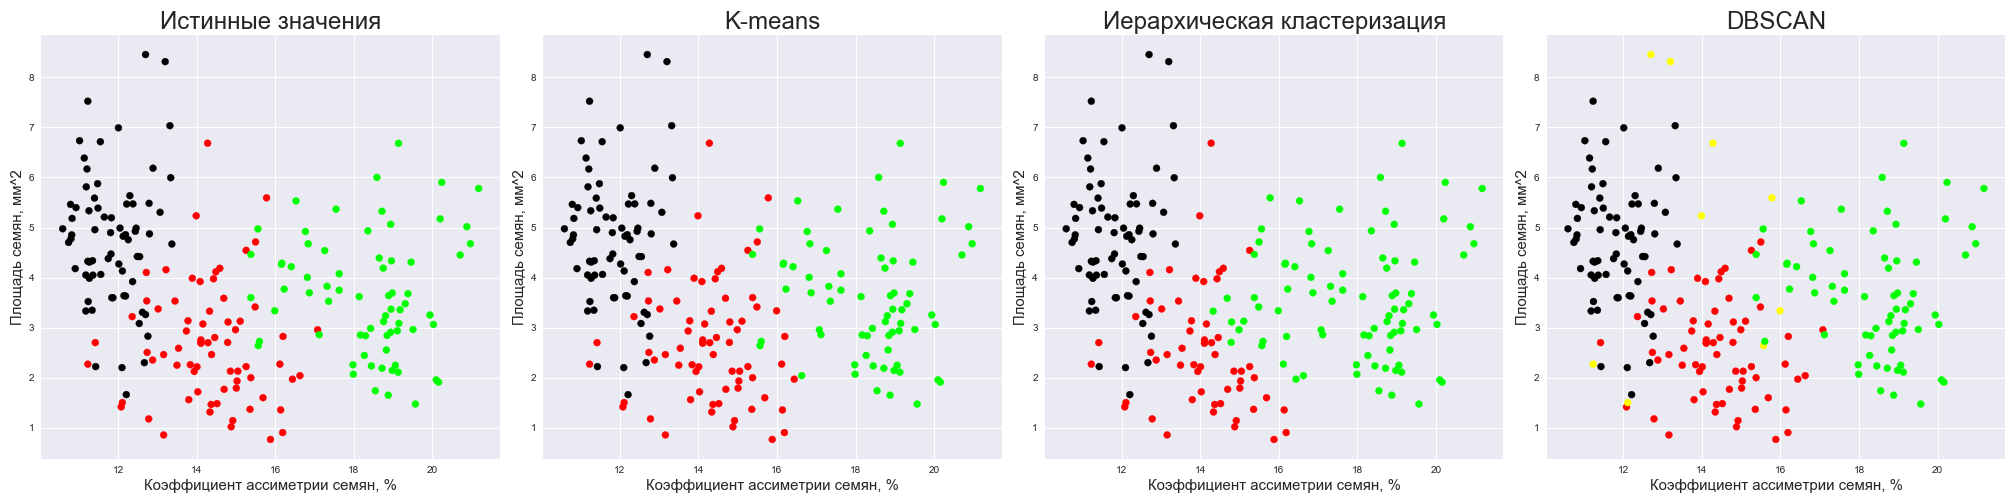
\includegraphics[width=4\linewidth]{plot.png}
\end{minipage}
\hfill


  {Боевая задача: 210 элементов в датасете, 3 сорта семян пшенницы: Kama, Rosa и Canadian. Цель алгоритмов –  разделить семена на виды по признакам после того, как мы отрезали столбик с верными ответами.}



Все алгоритмы практически верно разделили объекты на кластеры, не зная правильного результата. Один лишь DBSCAN отстал от своих собратьев и впопыхах выделил несколько объектов в класс выбросов (отмечены жёлтым).

 \innerblock[]{Код работы}{Вы можете посмотреть код работы и оценить прочие вкусняшки на github.com/PereverzevVV}
}
\end{columns}

\end{document}